\subsection{DOM}
Rečeno je da je $JavaScript$ služi za davanje interaktivnosti stranici, međutim, do sad smo sve ispisivali u konzoli sa malo interakcije sa stranicom. Da bismo mogli da dodamo interaktivnost sa postojećim elementima stranice (ili da kreiramo nove) moramo najpre naučiti kako da tim elementima pristupimo. Za svaku web stranicu pregledač formira nešto što nazivamo \textbf{DOM}\footnote{engl. Document Object Model}. DOM je drvolika struktura čiji su elementi $HTML$ elementi (tagovi) i njihovi sadržaji(unutar tagova). $DOM$ čuva hijerarhijsku strukturu u smislu da je neki element, koji je u $HTML$-u bio roditeljski element nekog drugog elementa, i u $DOM$-u roditeljski element. Elementi koji su hijerarhijski $"$ispod$"$ nekog elementa nazivamo decom ili, ako je u pitanju jedan element, detetom (engl. child). Koren $DOM$ stabla je objekat $window$ koji predstavlja prozor pregledača. Elementi napisani u $HTML$-u odgovaraju čvorovima podstabla čiji je koren objekat $document$, jedan od sinova objekta $window$. Pogledajmo sliku:
\begin{figure}[h!]
\begin{center}
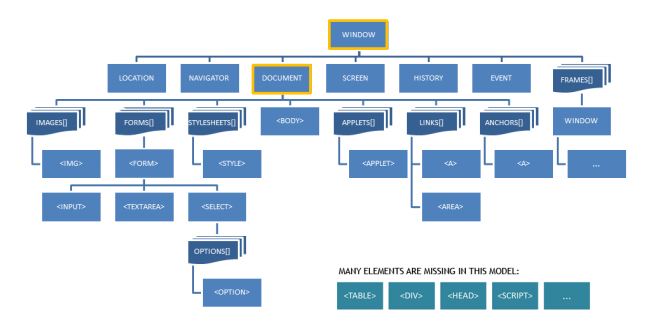
\includegraphics[scale=0.5]{../pictures/structure.png}
\end{center}
\caption{Prikaz DOM stabla počevši od window objekta.}
\label{fig:domwin}
\end{figure}
\subparagraph{Vežba}  Izabrati sajt i kreirati strukturu $DOM$ stabla. Kao na primeru:
\begin{lstlisting}[backgroundcolor = \color{lightgray}, breaklines=true]
<div>
 <h1>Ovo je naslov</h1>
 <h2>Ovo je podnaslov</h2>
</div>
\end{lstlisting} 	 
\begin{figure}[h!]
\begin{center}
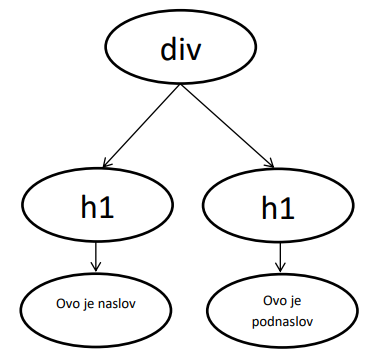
\includegraphics[scale=0.5]{../pictures/dom.png}
\end{center}
\caption{Prikaz primera DOM stabla.}
\label{fig:dom}
\end{figure}	  
\subsubsection{Osnove}
Kao što je ranije rečeno $JavaScript$ je skript jezik čija je osnovna uloga na Veb-u programiranje korisničkog interfejsa. Korišćenje jezika Javascript omogućava interakciju sa DOM stablom,
njegovo menjanje i obilaženje. Sve izmene napravljene nad čvorovima DOM stabla biće
vidljive na stranici u okviru elemenata čiji su odgovarajući čvorovi DOM-a menjani.
Naglasimo još jednom da programi napisani jezikom $JavaScript$ se izvršavaju na klijentskoj mašini (iako postoje i upotrebe na serveru).\\\\
Dohvatanje $DOM$ elemenata vrši se funkcijama definisanim u interfejsu $document$. Neke od najvažnijih navedene su u nastavku:
\begin{itemize}
\item \textbf{document.getElementsByTagName()} - dohvatanje elemenata čiji je naziv etikete (tag-a) prosleđen kao argument funkcije. Funkcija vraća niz objekata(čvorova stabla) koji odgovaraju pronađenim elementima. Niz je, kao i obično, indeksiran počevši od 0.
\item \textbf{document.getElementById()} - dohvatanje elementa čiji je $id$ prosleđen kao argument.
\item \textbf{document.getElementsByClassName()} - dohvatanje elemenata čiji je naziv klase prosleđen kao argument funkcije. Funkcija vraća niz objekata(čvorova stabla) koji odgovaraju pronađenim elementima. Niz je, kao i obično, indeksiran počevši od 0.
\item \textbf{document.getElementsByName()} -dohvatanje elemenata čija je vrednost atributa $name$  prosleđena kao argument funkcije. Funkcija vraća niz objekata(čvorova stabla) koji odgovaraju pronađenim elementima. Niz je, kao i obično, indeksiran počevši od 0.
\item \textbf{document.querySelector()} - dohvatanje elemenata CSS selektorom navedenim kao argument funkcije. Ukoliko ih je više, vraća samo prvi. 
\item \textbf{document.querySelectorAll()} - isto kao ponaša se isto kao $querySelector()$, osim što vraća niz svih objekata koji odgovaraju postavljenom kriterijumu. Niz je, kao i obično, indeksiran počevši od 0.
\end{itemize}
\begin{lstlisting}[backgroundcolor = \color{lightgray}, mathescape=true]
HTML:
<p class='pasus'>Neki pasus</p> 
<h1> Naslov nakon prvog pasusa</h1>
<div id='omotac'>
	<p class='pasus' id='pasus1'>Prvi pasus</p> 
	<p class='pasus' id='pasus2'>Drugi pasus</p>
	<p class='pasus' id='pasus3'>Treci pasus</p>
</div>

JS:
var omotac_element = document.getElementById("omotac");
var svi_pasusi = document.getElementsByTagName('p');
var pasusi_u_omotacu = document.querySelectorAll('#omotac .pasus'); // 
var prvi_pasus = document.querySelector('#omotac .pasus');
var drugi_pasus = document.querySelector('p:nth-child(2)');
var treci_pasus = pasusi_u_omotacu[2];
\end{lstlisting} 	 
Treba obratiti pažnju da se nazivi tagova navode između navodnika. Osim njih, uslove navodimo između navodnika. Primetimo da se uslovi mogu postavljati korišćenjem istih oznaka kao u $CSS$-u, pa tako uslov $'\#omotac\ .pasus'$ tumači se kao: $"$u elementu sa $id$-jem $omotac$ pronađi sve elemente koji pripadaju klasi pasus. $"$
Svojstvima dohvaćenog elementa pristupa se uz pomoć tzv. \textbf{tačka notacije}, što znači da nakon naziva promenljive, navodimo tačku, a potom ime svojstva. Sadržaj unutar etiketa $HTML$ elementa nalazi se u svojstvu $innerHTML$ objekta koji odgovara dohvaćenom elementu. Sadržaj ima tip niske.
\begin{lstlisting}[backgroundcolor = \color{lightgray}, breaklines=true]
HTML:
<p id='pasusneki'>Neki<a href=''>link</a> pasus</p>

JS:
var sadrzaj = document.getElementById('pasusneki').innerHTML;
console.log(sadrzaj);
\end{lstlisting} 	 
Da bismo pristupili tekstualnom sadržaju nekog elementa koristimo svojstvo $textContent$.
\begin{lstlisting}[backgroundcolor = \color{lightgray}, breaklines=true]
HTML:
<p id='pasusneki'>Neki <a href=''>link</a> pasus</p>

JS:
var sadrzaj = document.getElementById('pasusneki').textContent;
console.log(sadrzaj);
\end{lstlisting}

Razlika između ova dva pristupa je što ćemo u prvom slučaju dobiti sav sadržaj unutar $<p>$ etiketa. U drugom slučaju, dobićemo samo tekstualni sadržaj kako je i prikazan na stranici. \\\\
Kada koristimo metode koje vraćaju više od jednog elementa, na primer $getElementsByTagName$, kako bismo saznali koliko je takvih elemenata možemo koristiti svojstvo $length$.
\begin{lstlisting}[backgroundcolor = \color{lightgray}, breaklines=true]
var broj_elemenata = svi_pasusi.length;
console.log(broj_elemenata);
\end{lstlisting}
Kako bismo pristupili pojedinačnom elementu koristimo notaciju kao kod nizova (pošto metod zapravo i vraća niz elemenata).
\begin{lstlisting}[backgroundcolor = \color{lightgray}, breaklines=true]
var pasus = svi_pasusi[0];
console.log(pasus);
var poslednji = svi_pasusi[broj_elemenata-1].textContent;
console.log(poslednji);
\end{lstlisting}

%Za pristupanje vrednostima $input$ elementa koristi se svojstvo $value$.
%\begin{lstlisting}[backgroundcolor = \color{lightgray}, breaklines=true]
%HTML:
%<input type='text' id='ime'>

%JS:
%var input_polje = document.getElementById('ime');
%var vrednost_polja = input_polje.value;
%console.log(vrednost_polja);
%\end{lstlisting} 	 
CSS svojstvima elementa pristupa se pomoću svojstva $style$. Ovo svojstvo nam dozvoljava da eksplicitno zadajemo, menjamo i očitavamo stilove. Objekat koji odgovara
svojstvu $style$ sadrži samo eksplicitno zadate CSS vrednosti, ne i one koje nisu
navedene CSS-om a koje je pregledač samostalno izračunao. Vrednosti CSS svojstva se
pristupa preko njenog naziva, ukoliko naziv sadrži crticu za pristup svojstvu se koristi
naziv u kome crtica ne postoji, ali je prvo slovo posle crtice u originalnom zapisu veliko
(npr. $background\-color  \rightarrow backgroundColor$). Izračunate CSS vrednosti dobijaju se
funkcijom $getComputedStyle$ iz interfejsa $windows$, element čija se izračunata svojstva
traže se prosleđuje kao argument funkcije. Novu vrednost nekog svojstva postavljamo uz pomoć $element.style.osobina = vrednost$. Možemo na ovakav način dodavati i nove klase elementima, koristeći svojstvo $className$.
\begin{lstlisting}[backgroundcolor = \color{lightgray}, breaklines=true]
var stil_pasusa = pasus.style;
console.log(stil_pasusa);
var izracunati_stil = window.getComputedStyle(pasus);
console.log(izracunati_stil.color);
stil_pasusa.backgroundColor = 'gray';
document.querySelector('#pasus1').style.fontSize = '12px';
document.querySelector('#pasus2').className = 'doterani_pasus';
\end{lstlisting} 	

Kada dohvatimo neki $HTML$ element, moguće je kretanjem kroz $DOM$ stablo doći i do ostalih elemenata prateći veze sa ostalim elementima. Roditeljskom elementu nekog elementa pristupa se preko svojstva $parentElement$, koja sadrži pokazivač na roditeljski element. Elementu na istom nivou $DOM$ stabla $brat$/$sestra$ elementa, koji u $HTML$ strukturi sledi nakon dohvaćenog pristupa se svojstvom $nextElementSibling$. Očekivano, njegovom prethodniku pristupa se sa $previousElementSibling$.\\\\
Na veoma sličan način možemo posmatrati i strukturu u odnosu na roditeljski element. Naime, prvom direktnom potomku roditeljskog elementa pristupa se sa $firstElementChild$, poslednjem sa $lastElementChild$. Svim direktnim potomcima se pristupa svojstvom $children$, koje sadrži niz objekata koji odgovaraju direktnim potomcima elementa. Pogledajmo kroz primer:
\begin{lstlisting}[backgroundcolor = \color{lightgray}, breaklines=true]
var omotac = document.getElementById('omotac');
var prvi_pasus = omotac.firstElementChild;
var drugi_pasus = prvi_pasus.nextElementSibling;
var treci_pasus = drugi_pasus.parentElement.lastElementChild;
var naslov = omotac.previousElementSibling;
\end{lstlisting} 	
Na slici \ref{fig:dom3} se vidi grafički prikaz.
\begin{figure}[h!]
\begin{center}
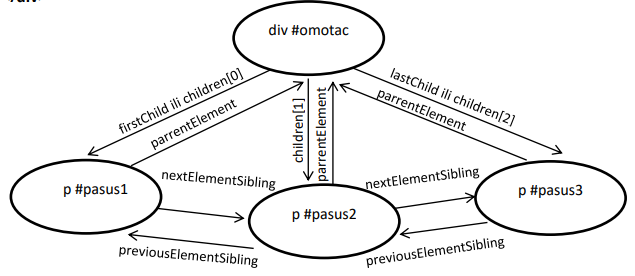
\includegraphics[scale=0.5]{../pictures/parentchild2.png}
\end{center}
\caption{Prikaz odnosa između elemenata u DOM stablu.}
\label{fig:dom3}
\end{figure}
Na slici \ref{fig:dom2} se na primeru liste jasno vide odnosi između elemenata:
\begin{figure}[h!]
\begin{center}
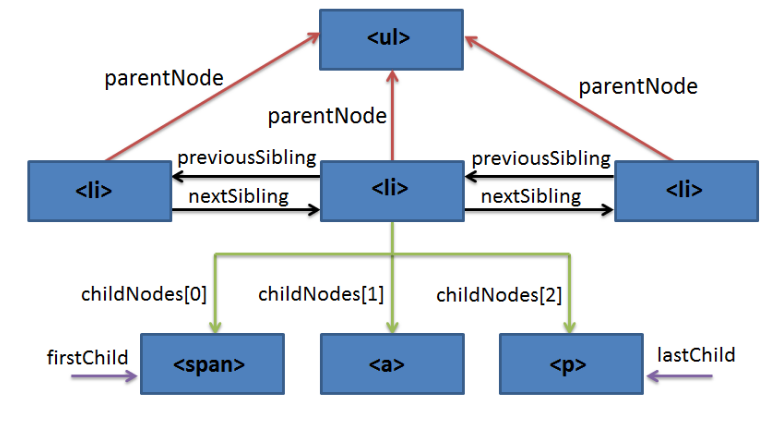
\includegraphics[scale=0.5]{../pictures/parentchild.png}
\end{center}
\caption{Prikaz odnosa između elemenata u DOM stablu.}
\label{fig:dom2}
\end{figure}	
Atributima dohvaćenih elemenata pristupa se funkcijom $getAttribute()$ kojoj se kao argument prosleđuje naziv atributa čija se vrednost traži. Postavljanje atributa elementima vrši se funkcijom $setAttribute()$ čiji je prvi argument naziv novog atributa, a drugi argument željena vrednost novog atributa.
\begin{lstlisting}[backgroundcolor = \color{lightgray}, breaklines=true]
HTML:
<p id='pasus' title='Neki naslov'>Neki pasus</p>

JS:
var pasus = document.getElementById('pasus');
var title = pasus.getAttribute('title');
console.log(title);
pasus.setAttribute('class', 'klasa1');
\end{lstlisting}

\subparagraph{Zadaci - DOM osnove }
\begin{primer}
Kreirati stranicu bioskopa koja sadrži $4$ $div$a. Prvi $div$ sadrzi naslov stranice i logo. Drugi $div$ sadrži sadržaj stranice (content, na primer, najave premijera). Treci $div$ sadrzi informacije poput kontakt telefona i ostalih informacija o cenama karata i datumima nekih od projekcija. Cetvrti div je footer u kome mogu biti smestene adresa preduzeca kao i polje za prijavu za $newsletter$. Pristupiti pasusu unutar drugog $div$-a promeniti mu pozadinu sa crvene na sivu. Dohvatiti sve naslove $h2$ i promeniti im boju na belu. Postaviti boju elementa sa $id$-jem "neki\_odabrani" na plavu. Za liste postaviti veličinu slova na $11px$. 
\end{primer}

\begin{primer}
Dohvatiti sve elemente liste unutar elementa sa $id$-jem $cenovnik$. Podesiti dohvaćenim elementima slova da budu iskošena, i promeniti boju na belo. Promeniti pozadinsku boju $cenovnika$ na ljubičasto.
\end{primer}

\begin{primer}
Za kreiranu stranicu koja sadrzi 10 pasusa, postaviti pozadinsku boju svakom drugom na svetlo sivu.
\end{primer}

\begin{primer}
Za stranicu sa bioskopom kreirati novi element koji u sebi sadrži 6 $div$-ova sa najavama budućih projekcija. Svaka od najava treba da sadrži naslov filma, poster, datum premijere, kratak opis i link ka detaljnijim informacijama. Treba promeniti boju prvom, poslednjem, kao i drugom i pretposlednjem elementu na: plavu (prvi i poslednji), svetlo plavu (drugi i pretposlednji). Preostala dva elementa treba da ostanu bela. Napomena: slobodno odabrati boje iz palete boja koje bi se uklopile sa vasim sajtom.   
\end{primer}

\begin{primer}
Na stranicu sa bioskopom postaviti tooltip sa tekstom $"$Gledajmo budućnost zajedno!$"$ na glavni naslov. Kreirati element koji sadrži naslov $"$Najpopularniji film u $2018$.$"$, poster i naziv filma. Postaviti atribute širine i visine slike koja predstavlja najpopularniji film na $100$ prema $150$px. Dohvatiti atribute vezane za linkove ka narednim projekcijama iz elementa koji sadrži najave i promeniti ih tako da predstavljaju linkove ka $IMDB$ stranicama filmova. Na kraju, za najpopularniji film, dodati ocenu i link ka $IMDB$ stranici.  
\end{primer}
\newpage

\subsubsection{Kreiranje elemenata}
Nekada ne želimo samo da menjamo postojeće elemente, već želimo i da kreiramo nove. Pravljenje novih elemenata vrši se funkcijom $createElement$ iz interfejsa $document$. Kao argument ova funkcija prima naziv etikete novog elementa (naziv etikete se navodi pod navodnicima). Element se vezuje u $DOM$ stablo kao poslednji sin nekog elementa funkcijom $appendChild$ čiji je argument element koji se u stablo dodaje. U slučaju da ne iskoristimo append child, element neće biti prikazan.

\begin{lstlisting}[backgroundcolor = \color{lightgray}, breaklines=true]
var omotac = document.getElementById('omotac');
var novi_pasus = document.createElement('p');
novi_pasus.innerHTML = "Treci pasus <a href=''>link</a>";
novi_pasus.setAttribute('id', 'pasus3');
//obavezno vezivanje novog pasusa kao poslednje dete omotaca
omotac.appendChild(novi_pasus);
\end{lstlisting}

Ukoliko zelimo da postavimo tekstualni sadržaj nad elementom, moramo napraviti novi tekstualni čvor sa $createTextNode$, a potom ga sa $appendChild$ dodati odgovarajućem elementu. Primetiti da sa $createTextNode$ takođe dodajemo tekst kao sa $innerHTML$. Razlika je u tome što će $innerHTML$ tumačiti etikete i prikazivati ih na odgovarajući način dok $createTextNode$ nece. Još jedna razlika koju možemo videti je ta da sa $innerHTML$ zamenjujemo celokupni sadržaj elementa novim sadržajem, dok sa $createTextNode$ dodajemo novi sadržaj na postojeći.

\begin{lstlisting}[backgroundcolor = \color{lightgray}, breaklines=true]
var cetvrti = document.createElement('p');
var sadrzaj = document.createTextNode("Cetvrti pasus <a href=''>link</a>");
cetvrti.appendChild(sadrzaj);
omotac.appendChild(cetvrti);

//createTextNode dodaje sadrzaj na postojeci
var pasus1 = document.getElementById('pasus1');
var sadrzaj = document.createTextNode('jos neki tekst unutar pasusa1');
pasus1.appendChild(sadrzaj);
//innerHTML zamenjuje sadrzaj u potpunosti
pasus1.innerHTML = "Tekst unutar pasusa1";
\end{lstlisting}

Dodavanjem novih elemenata sa $appendChild$, uvek dodajemo element kao poslednjeg naslednika u nizu elementa na koji vršimo $"$lepljenje$"$. Ako bismo želeli da dodamo novi element pre nekog drugog elementa koristimo $insertBefore()$. Ova funkcija prima dva argumenta. Prvi, novokreirani čvor, koji želimo da ubacimo pre drugog argumenta, koji predstavlja neki postojeći čvor. 
\begin{lstlisting}[backgroundcolor = \color{lightgray}, breaklines=true]
var pasus_jedan_ipo = document.createElement('p');
var pasus2 = document.getElementById('pasus2');
pasus_jedan_ipo.innerHTML = "pasus i po";
omotac.insertBefore(pasus_jedan_ipo, pasus2);
\end{lstlisting}

Da bismo jedan element-dete zamenili drugim, koristimo metod $replaceChild()$. Ovaj metod prima iste argumente kao i $insertBefore()$.

Ako želimo da obrišemo neki element koristimo $removeChild$. Sa $document.body$ pristupamo elementima koji se nalaze unutar $<body>$ etiketa.
\begin{lstlisting}[backgroundcolor = \color{lightgray}, breaklines=true]
HTML:
<p id='obrisi'>Pasus koji zelimo da obrisemo</p>
JS:
var obrisi = document.getElementById('obrisi');
document.body.removeChild(obrisi);
\end{lstlisting}
\subparagraph{Zadaci - Kreiranje elemenata}
\begin{primer}
Na stranicu sa pozorištem dodati nove elemente. Elemente dodavati kreiranjem novih elemenata kroz $JavaScript$. Obavezno dodati tabelu, sliku, link, dok su ostali elementi po izboru u zavisnosti od rada.
\end{primer}

\begin{primer}
Kreirati stranicu na kojoj se nalazi samo jedan prazan $div$ sa $id$-jem $omotac$. U taj $div$, dodavati elemente korišćenjem funkcije $createElement$ dok se ne dobije stranica koja sadrži rezultate ispita. Stranica treba da sadrži barem naslov i tabelu sa spiskom učenika i njihovim ocena koji se izvlači iz objekta.
\end{primer}

\begin{primer}
Za uneti ceo broj $n$, izgenerisati tablicu množenja veličine $n$ koristeći table element i dodavanje uz pomoć interakcije sa DOM drvetom. Doterati stranicu koristeći CSS.
\end{primer}

\begin{primer}
Kreirati sajt koji će sadržati biografije do 3 znamenita naučnika. Na osnovu naziva slike koji se unosi preko prompta, dodati na stranicu primer biografije zadate ličnosti. Na primer, za naziv slike $tesla.jpg$ na stranicu dodati naslov Nikola Tesla, paragraf sa kratkom biografijom, sliku, kao i link ka stranici na Wikipediji. Svaka biografija treba da bude prigodno uokvirena. Ponuditi unos za do 3 licnosti, tako sto ce se preko prompta najpre uneti broj licnosti, a potom i nazivi slika koje korisnik želi da iskoristi pri kreiranju stranice. Sajt ukrasiti korišćenjem prigodinih HTML i CSS elemenata.
\end{primer}

\begin{primer}
Kreirati stranicu koja vrši heširanje tajne poruke koju korisnik unosi preko prompta. Heširanje predstavlja postupak sakrivanja poruke. U ovom zadatku heš treba predstaviti preko tabele, koja u vidu niza predstavlja poruku uz pomoć crvenih, plavih i zelenih kvadratića dimenzija 10x10 piksela. Heš funkcija je sledeća:
\begin{itemize}
\item ako je ostatak pri deljenju kodnog broja karaktera sa 3 jednak 1 onda zelena boja,
\item ako je ostatak pri deljenju kodnog broja karaktera sa 3 jednak 2 onda plava boja
\item inače, crvena. 
\end{itemize}
Prikaz programa dat je na slici \ref{fig:hes}.
\begin{figure}[h!]
\begin{center}
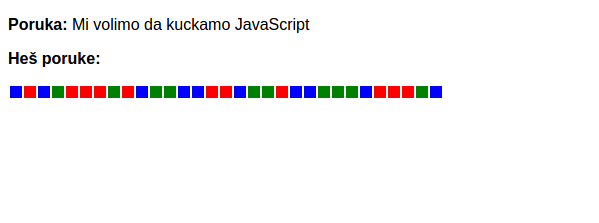
\includegraphics[scale=0.5]{../pictures/hes.png}
\end{center}
\caption{Prikaz programa.}
\label{fig:hes}
\end{figure}

\end{primer}
\newpage

\subsubsection{Reagovanje na događaje}
Na način na koji smo do sada vršili interakciju sa stranicom još uvek nismo mogli da dobijemo pravu interaktivnost. Da bismo to postigli neophodno je da vršimo interakciju sa elementima DOM-a.
Svaka interakcija sa elementima DOM-a predstavlja događaj. Događaj predstavljaju različite interakcije korisnika sa stranicom kao što su: klik, prelazak miša, pritisak određenih tastera, itd..Prilikom pojave događaja moguće je reagovati i izvršiti određene naredbe. Da bi se pojava nekog događaja vezala sa akcijom koju je potrebno preduzeti potrebno je prijaviti se, odnosno, „osluškivati“ pojavu nekog događaja.  Postoje dva načina da osluškujemo događaje. Prvi način za to je navođenje odgovarajućeg atributa elementa na kome se događaj očekuje. Takvi atributi obavezno imaju prefix $on$ nakon koga se nastavlja naziv događaja. Na primer, ako je naziv događaja $click$, atribut će imati naziv $onclick$. Vrednost atributa je naziv funkcije koju je potrebno izvršiti ukoliko se događaj desio. Obratiti pažnju da se naziv funkcije šalje sa zagradama i da naziv događaja ima prefiks $on$. Element na kome se događaj dogodio može se dohvatiti korišćenjem ključne reči $this$. Nakon $this$ možemo navesti bilo koje od svojstava objekata, npr. $value$ ($this.value$). Napomena: Ovaj način se manje preporučuje, jer meša opis stranice ($HTML$) i ponašanje stranice ($JavaScript$). 
\begin{lstlisting}[backgroundcolor = \color{lightgray}, breaklines=true]
HTML:
<button onclick='prikaziObavestenje()'>Prikazi obavestenje</button>
JS:
function prikaziObavestenje(){
  alert("Obavestenje prikazano klikom na dugme " + this.innerHTML);
}
\end{lstlisting}
Neki od atributa koji postoje su: 
\begin{itemize}
\item \textbf{onclick} - definiše šta se događa kada korisnik klikne na površinu elementa 
\item \textbf{ondblclick} - definiše šta se događa kada korisnik dva puta klikne za redom
\item \textbf{onmouseover} - definiše šta se događa kada korisnik pređe mišem preko elementa
\item \textbf{onkeyup} - definiše šta se događa kada korisnik pusti pritisnuti taster na tastaturi 
\item \textbf{onchange} -  definiše šta se događa kada korisnik promeni vrednost npr. input elementa ili select elementa
\item \textbf{onfocus} - definiše šta se događa kada element dobije fokus (kada se korisnik pozicionira bilo mišem bilo tab tasterom na ovo polje)
\item \textbf{onblur} - definiše šta se događa kada element izgubi fokus
\item \textbf{onhover} - definiše šta se događa kada se pređe preko površine elementa 
\item \textbf{onkeyup} - definiše šta se događa kada korisnik pritisne taster na tastaturi (spust tastera)  
\end{itemize}                        
 
Pogledajmo nesto detaljniji primer:
\begin{lstlisting}[backgroundcolor = \color{lightgray}, breaklines=true]
HTML:
<h2> Preko HTML atributa</h2>
<br>
<button onclick='prikaziObavestenje()'>Prikazi</button>
<br>
<div id='ip'>
  <h2>This</h2>
  <input type='text' id='ime' onblur="unos(this.value)">
  <button id='dugme3' onclick='podatak()'>Konzola</button>
  <p id="paragraf"></p>
  <br>
</div>

JS:
function prikaziObavestenje(){
  alert("Obavestenje prikazano klikom na dugme.");
}

function podatak(){
  var vrednost_polja = input_polje.value;
  console.log(vrednost_polja);    
}
//ova funkcija kao argument prima this.value 
//koji predstavlja vrednost unosa
//tu vrednost zelimo da ispisemo
function unos(tekst){
  var par = document.getElementById('paragraf');
  par.innerHTML = tekst;
  par.style.backgroundColor = 'lightblue';
}           
\end{lstlisting} 

Primetimo da se u kodu pojavljuje $this$. $this$ prilikom gore navedenog navodjenja predstavlja ceo input element, pa se moze pristupiti svim njegovim svojstvima - u ovom slučaju se funkciji $prikazi$ prosleđuje tekući tekstualni sadržaj elementa.\\\\

Drugi način osluškivanja događaja je dodavanje „osluškivača“ ($listener$-a) u okviru
$JavaScript$ koda na element na kome se događaj očekuje, korišćenjem funkcije
$addEventListener()$. Ova funkcija prima dva argumenta. Prvi je naziv događaja čija se
pojava osluškuje, a drugi je naziv funkcije koja će se pozvati kada se događaj desi. Moguće je kao drugi argument navesti i anonimnu funkciju koja će biti definisana odmah na mestu argumenta. Obratiti pažnju da se naziv funkcije šalje bez ikakvih zagrada, a da naziv događaja nema prefiks $on$. Da bismo uopšte mogli da postavimo osluškivač događaja na neki element moramo ga najpre dohvatiti.
\begin{lstlisting}[backgroundcolor = \color{lightgray}, breaklines=true]
HTML:
<button id='dugme1'>Dugme1</button>
<button id='dugme2'>Dugme2</button>
JS:
var dugme1 = document.getElementById('dugme1');
var dugme2 = document.getElementById('dugme2');
dugme1.addEventListener('click', prikaziObavestenje);
dugme2.addEventListener('mouseover', function(){
  alert("Obavestenje iz anonimne funkcije");
});
\end{lstlisting}

Neki od događaja na koje se može reagovati su:
\begin{itemize}
\item \textbf{click} – klik na element
\item \textbf{dblclick} – dupli klik na element
\item \textbf{focus}  – dovođenje elementa u fokus (klikom, dugmetom tab, programski...)
\item \textbf{blur} – promena fokusa sa fokusiranog elementa na drugi element
\item \textbf{mouseenter}  – ulaz kursora u okvir elementa
\item \textbf{mouseover} – pomeranje kursora preko elementa
\item \textbf{mouseleave} – izlaz kursora iz okvira elementa
\item \textbf{onload} – pri završenom učitavanju elementa (iscrtavanju i smeštanju u DOM)
\item \textbf{keypress}  – Pritisnuto je dugme na tastaturi dok je element u fokusu, objekat prosleđen kao argument funkciji za obradu događaja sadrži informacije o tome koje dugme je
pritisnuto
\end{itemize}
Pogledajmo i ovde nešto detaljniji primer:
\begin{lstlisting}[backgroundcolor = \color{lightgray}, breaklines=true]
HTML:
<p>Unesite tekst (kada element izgubi fokus prikazace se njegov sadrzaj): </p>
<input type='text' id='unos2'> 
<br>
<p>Unesite karakter ciji kodni broj zelite:</p>
<textarea id='tekstualno'></textarea>

JS:
var input_polje = document.getElementById('ime');
var vrednost_polja = input_polje.value;
console.log(vrednost_polja);

document.querySelector('#unos2').onblur=function(){            
  window.alert("Novi sadrzaj je: " + this.value);
}
            
var tekstualno_polje = document.getElementById('tekstualno');
// U zavisnosti od pregledaca, kodni broj karaktera se dobija
// koriscenjem funkcija which ili keycode
tekstualno_polje.addEventListener('keypress',function(dogadjaj){
  alert("Pritisnuto je dugme sa kodom:" + (dogadjaj.which || dogadjaj.keycode))
});
\end{lstlisting} 

U ovom primeru koristili smo $keypress$. On označava da je pritisnuto dugme na tastaturi dok je element u fokusu. Objekat prosleđen kao argument funkciji za obradu događaja sadrži informacije o tome koje dugme je pritisnuto.

Svi navedeni događaji mogu biti korišćeni i kao atributi i kao argumenti funkcije. U prvom slučaju treba koristiti prefiks $on$. Za kompletnu listu ovih događaja konsultovati dodatnu literaturu.

\subparagraph{Zadaci - Reagovanje na događaje}

\begin{primer}
Kreirati sajt "Mala škola programiranja". Sajt treba da sadrži:
\begin{itemize}
\item pozadinsku sliku
\item navigacioni bar (pocetna kursevi kontakt)
\item na početnoj strani treba da se nalazi malo polje sa pitanjem $"$Da li volite da
     programirate?$"$, a ispod toga dva button-odgovora na pitanje $DA$ i $NE$ 
\item klikom na dugme DA izbacuje se alert sa natpisom "Svaka cast! Buducnost je Vasa!"
\item prelaskom miša preko dugmeta NE, dugme treba da pobegne na proizvoljni deo ekrana
    (koristiti funkciju Random ---> Math.Random())
\item sajt je neophodno ukrasiti odgovarajucim CSS elementima. 
\end{itemize}
\end{primer}

\begin{primer}
Kreirati igru $X$-$O$. Igra se sastoji iz table $3$x$3$. Naizmenično se unose $X$ i $O$ (klikom) dok se u bilo kom smeru ne nađu tri uzastopna ista znaka. Na kraju se ispisuje obaveštenje o tome koji igrač je pobedio i $"$Nerešeno!$"$ ako je rezultat nerešen.
\end{primer}


\begin{primer}
Skočko - Kreirati igru koja je poput igre skočko iz kviza $"$Slagalica$"$. Nasumično se generišu 4 simbola od 6 mogućih. Potom se korisniku nudi da unese odgovarajuće
\end{primer}

\begin{primer}
Kreirati stranicu koja se sastoji iz 4 raznobojna dugmeta kreirana kroz CSS. Stranica predstavlja kulturni vodič kroz grad. Stranica treba da sadrži naslov $"$Kulturni vodič kroz grad$"$, a potom ispod treba da piše odaberite tip događaja. Prelaskom kursora preko dugmeta treba da se promeni boja dugmeta u svetliju nijansu dodeljene boje. Dugmici treba da sadrže naslove: bioskop, pozoriste, muzej, koncert. Klikom na dugme otvara se odgovarajuća stranica. Za stranicu o muzeju modifikovati stranicu sa biografijama najvećih srpskih naucnika tako da ona predstavlja deo prezentacije muzeja. Stranicu o koncertima treba kreirati korišćenjem niza događaja koji bi dodavali različite elemente stranice. 
\end{primer}
\newpage

\subsubsection{Validacija formi}
Forme predstavljaju jedan od osnovnih vidova prikupljanja određenih podataka koje korisnik unosi. Da bi se informacije prikupile i sačuvale, podaci se šalju na server. Da ne bi došlo do toga da korisnik unosi besmislice veoma nam je važna validacija formi, odnosno, onoga što korisnik unosi.
Vrlo često želimo da analiziramo korisnički unos i pre nego što podatke pošaljemo na server. Time možemo da izbegnemo da se neispravni podaci šalju uopšte do servera, a potom da se vraća sa servera informacija da nešto nije u redu. Taj prvi nivo filtracije podataka vrši se upravo kroz $JavaScript$. Za pristupanje vrednostima input elemenata koristi se svojstvo $value$.
\begin{lstlisting}[backgroundcolor = \color{lightgray}, breaklines=true]
HTML:
<input type='text' id='ime'>
<button id='dugme3' onclick='podatak()'>Konzola</button>
JS:
function podatak(){
	var vrednost_polja = input_polje.value;
	console.log(vrednost_polja);    
}
var input_polje = document.getElementById('ime');
var vrednost_polja = input_polje.value;
console.log(vrednost_polja);
\end{lstlisting}
Primetiti da ako uradimo $console.log(vrednost\_polja)$ van funkcije ne dobijamo ništa. To je posledica toga što u momentu kada se taj deo koda izvršava još uvek nije uneto ništa. Sa druge strane, ako bismo uneli neki tekst i potom klikom na dugme $Konzola$, pozvali funkciju $podatak()$, dobijamo ono što je uneto.\\\\

Postoji događaj koji se odnosi na forme, a to je $submit$. Ovaj događaj označava da treba poslati podatke iz formulara. Ukoliko je povratna vrednost funkcije koja se izvršava pri pojavi ovog događaja $false$ podaci neće biti poslati. Koristi se pri validaciji
formulara. \\\\
\begin{lstlisting}[backgroundcolor = \color{lightgray}, breaklines=true]
HTML:
<form onsubmit='return validacija()'>
...
</form>
JS:
function validacija(){

if(formaValidna)
  return true;
else
  return false;
}
\end{lstlisting}
Događaj koji nam pomaže da uhvatimo promenu vrednosti $input$ polja, odabrane vrednosti $select$ elementa ili elementa $textarea$ je $change$. Indeks odabrane opcije select elementa je vrednost svojstva $selectedIndex$.
\begin{lstlisting}[backgroundcolor = \color{lightgray}, breaklines=true]
HTML:
<select id='selekcija'>
	<option value='vrednost1'>Vrednost 1</option>
    <option value='vrednost2'>Vrednost 2</option>
</select>
JS:
var selekcija = document.getElementById('selekcija');
selekcija.addEventListener('change',function(){     
  console.log( "Odabrana je vrednost sa indeksom ",
  this.selectedIndex, " i vrednost je:", this.value);
});
\end{lstlisting}
Postoji i događaj $reset$ koji se aktivira prilikom poništavanja unetih polja. 

Najpre, da bismo prikupili informacije koje želimo da validiramo na raspolaganju nam je veliki broj HTML elemenata formulara. Neki od njih su:
\begin{itemize}
\item \textbf{input} - Prikaz ovog elementa zavisi od njegovog $type$ atributa:
	\begin{enumerate}
		\item \textbf{text} - jednolinijski tekst
		\begin{lstlisting}[backgroundcolor = \color{lightgray}, breaklines=true]
<input type='text'>
		\end{lstlisting}
		\item \textbf{password} - unos lozinke
		\begin{lstlisting}[backgroundcolor = \color{lightgray}, breaklines=true]
<input type='password'>
		\end{lstlisting}		
		\item \textbf{button} - proizvoljno dugme (može i preko elementa button)
		\begin{lstlisting}[backgroundcolor = \color{lightgray},breaklines=true]
<input type='button' value='Klikni!' onclick='alert("Hello World!)'>
		\end{lstlisting}
		\item \textbf{submit} - dugme koje šalje podatke ka serveru (samo u okviru form elementa)
		\item \textbf{reset} - dugme koje briše sve podatke unete u formular
		\item \textbf{radio} - dugme, ide u grupama dugmića istog tipa, nudi se odabir tačno jednog od ponuđenih. Neophodno je navođenje atributa $name$ za ovaj tip elementa, kako bi se znalo kojoj grupi pripada (grupisanje $radio$ dugmića). Dodavanjem atributa $value$ definišemo izbor opcije.
		\begin{lstlisting}[backgroundcolor = \color{lightgray}, breaklines=true]
<form>
  <input type='radio' name='pol' value='muski' checked>Muski
  <input type='radio' name='pol' value='zenski' checked>Zenski
  <input type='radio' name='pol' value='ostalo' checked>Ne zelim da odgovorim
</form>
		\end{lstlisting}
		\item \textbf{checkbox} - dugmići koji nude odabir više opcija, razlika u odnosu na prethodni je što ne moramo vršiti grupisanje.
		\begin{lstlisting}[backgroundcolor = \color{lightgray}, breaklines=true]
<form>
  <input type='checkbox' name='nivo1' value='srednja' checked>Srednja skola
  <input type='checkbox' name='nivo2' value='osnovne' checked>Osnovne studije
  <input type='checkbox' name='nivo3' value='master' checked>Master studije
</form>
		\end{lstlisting}
		\item Postoji još vrednosti za tip $input$-a, za više, posetiti:\href{https://www.w3schools.com/html/html_form_input_types.asp	}{W3Schools}
	\end{enumerate}
 	 Za element $input$ definisani su atributi:
 	 \begin{itemize}
 	 \item $name$ - za naziv opcije, 
 	 \item $value$ - za vrednost,
 	 \item $readonly$ - polje je samo za čitanje, vrednost ne bi trebalo da se menja, 
 	 \item $size$ - veličina polja u karakterima, 
 	 \item $maxlength$ - najveći broj karaktera koje element prima,
 	 \item $disabled$ - nije moguće unošenje u polje,
 	 \item $placeholder$ - vrednost postavljena pre unosa,
 	 \item $required$ - označava da zahtevamo da nešto bude uneseno u to polje (ovaj atribut nam ne obezbeđuje da će taj unos biti i ispravan!).
	\end{itemize} 	    
\item \textbf{select} - Ovaj element predstavlja padajuću listu sa izborima, sa atributom $name$ označavamo naziv te liste, a sa elementima $option$ opcije. Ako nad $select$-om postavimo atribut $multiple$ onda dozvoljavamo odabir više opcija.  
\item \textbf{option} - Predstavlja elemente padajuće liste. Ima atribut $value$ koji predstavlja vrednost izbora. Atributom $selected$ postavljamo podrazumevanu vrednost.
\begin{lstlisting}[backgroundcolor = \color{lightgray}, breaklines=true]
<select name="kursevi" multiple>
  <option value="engleski">Engleski</option>
  <option value="spanski">Spanski</option>
  <option value="francuski">Francuski</option>
  <option value="nemacki" selected>Nemacki</option>
</select>
\end{lstlisting}
\item \textbf{optgroup} - Dozvoljava grupisanje opcija.
\begin{lstlisting}[backgroundcolor = \color{lightgray}, breaklines=true]
<select name="kursevi" multiple>
<optgroup label='radnidani'>
  <option value="engleski">Engleski</option>
  <option value="spanski">Spanski</option>
</optgroup>
<optgroup label='vikend'>  
  <option value="francuski">Francuski</option>
  <option value="nemacki" selected>Nemacki</option>
</optgroup>
</select>
\end{lstlisting}
\item \textbf{textarea} - unos teksta u više linija. Ima atribute $rows$ i $cols$ koji označavaju broj redova i kolona koje je moguće uneti. Visina i širina ovog elementa mogu se izmeniti uz pomoć $CSS$-a.\\
\begin{lstlisting}[backgroundcolor = \color{lightgray}, breaklines=true]
<textarea name="biografija" rows="20" cols="30">
Napisite kratku biografiju.
</textarea>
\end{lstlisting}
\item \textbf{datalist} - Ako bismo hteli da napravimo $input$ polje koje bi nam nudilo više opcija ili radilo $autocomplete$ mogli bismo da atributu $list$ dodelimo naziv $id$ atributa elementa $datalist$. Potom u nastavku koristeći element $option$ navodimo moguće vrednosti atributom $value$.
\begin{lstlisting}[backgroundcolor = \color{lightgray}, breaklines=true] 	 
<input list="browsers">
<datalist id="browsers">
  <option value="Internet Explorer">
  <option value="Firefox">
  <option value="Chrome">
  <option value="Opera">
  <option value="Safari">
</datalist>
\end{lstlisting}
\item \textbf{fieldset} - grupisanje više elemenata forme u jednu celinu
\item \textbf{legend} - davanje naziva celini koja je izdvojena uz pomoć $fieldset$ elementa
\item \textbf{label} - daje semantičko značenje elementima forme, kada korisnici kliknu na labelu, onaj element koji je povezan sa tom labelom postaje aktivan. Da bismo izvršili povezivanje koristimo atribut $for$ koji dobija za vrednost naziv identifikatora onog elementa za koji labelu vezujemo.
\end{itemize}

Pogledajmo sada primer. Želimo da kreiramo formular kao na slici \ref{fig:formular}
\begin{figure}[h!]
\begin{center}
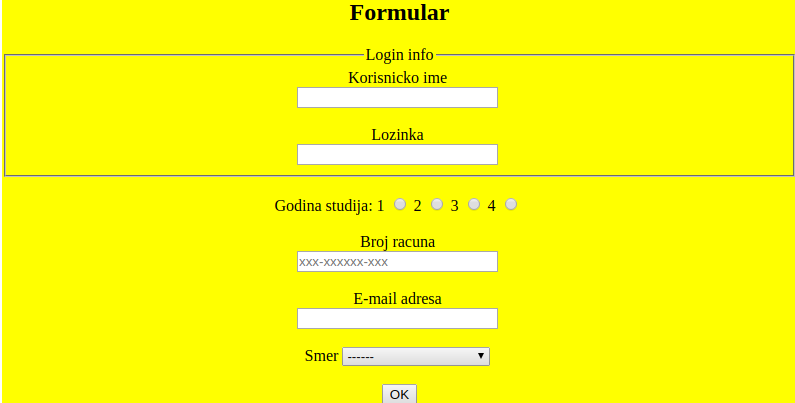
\includegraphics[scale=0.5]{../pictures/formular.png}
\end{center}
\caption{Prikaz primera formulara koji želimo da napravimo.}
\label{fig:formular}
\end{figure}	  

\begin{lstlisting}[backgroundcolor = \color{lightgray}, breaklines=true]
HTML:
<h2> Formular </h2>
<form id="forma" onsubmit="return provera()">
 <p id="greska" style="color: red"></p>
 <fieldset>
  <legend> Login info </legend>
  <label for="korisnickoIme">Korisnicko ime</label>
  <br>
  <input type="text" id="korisnickoIme" name="ime">
  <br>
  <br>
  <label for="lozinka">Lozinka</label>
  <br>
  <input type="password" name="pass" id="lozinka">
  <br>    
 </fieldset>
 <br>
 
 Godina studija:
 <label for="prva">1</label>
 <input type="radio" name="godina" id="prva" value="1">
 <label for="druga">2</label>
 <input type="radio" name="godina" id="druga" value="2">
 <label for="treca">3</label>
 <input type="radio" name="godina" id="treca" value="3">
 <label for="cetvrta">4</label>
 <input type="radio" name="godina" id="cetvrta" value="4">
 <br>

 <label for="racun">Broj racuna</label>
 <br>
 <input type="text" name="racun" id="racun" placeholder="xxx-xxxxxx-xxx">
 <br>
 
 <label for="email">E-mail adresa</label>
 <br>
 <input type="text" name="email" id="email">
                
 <br>
 <label for="smer">Smer</label>
 <select name="smer" id="smer">
  <option value="X">------</option>
  <option value="I">Informatika</option>
  <option value="M">Teorijska matematika</option>
  <option value="L">Profesorski</option>
 </select>
 <br>
 <input type="submit" value="OK">
</form>
\end{lstlisting}

Ovim delom koda smo omogućili korisniku da unese neke podatke.
Sada želimo da vidimo da li je ono što je uneto ispravno, i da, ako nije, ispišemo grešku.
\begin{lstlisting}[backgroundcolor = \color{lightgray}, breaklines=true]


\end{lstlisting}
Napomena: ovaj deo teksta ce biti prepravljen sa dodatnim objasnjenjima funkcija.

\subparagraph{Zadaci - Formulari i validacija}

\begin{primer}
Kreirati $"$Mirror$"$ sajt za izvrtanje korisnickog unosa. Pozadinska slika bi trebalo da bude
ogledalo. Kucanjem teksta u input polje istovremeno u paragrafu ispod se ispisuje tekst u 
obrnutom poretku. Sajt ukrasiti odgovarajucim CSS elementima.
\end{primer}

\begin{primer}
Kreirati stranicu na kojoj se unete rečenice (kroz textarea) sortiraju po dužini i ispisuju.
\end{primer}

\begin{primer}
Kreirati igru vešala. Najpre se unosi skrivena reč, na osnovu koje se formiraju polja. Potom se na neki od dva načina nudi korisniku da odabere slovo:
\begin{itemize}
\item unosom kroz polje ili
\item klikom na polje sa slovom.
\end{itemize}

\end{primer}

\begin{primer}
Modifikovati prethodni zadatak, tako da se korisniku ponudi najpre odabir lakše ili teže varijante igre. Ako je odabrana lakša verzija igra se odigrava kao u prethodnom zadatku.  Ako je odabrana teža verzija igra se modifikuje tako da se korisnik stavlja u vremensko ograničenje od 30, 45 ili 60 sekundi i broj pokušaja mu se ograničava na polovinu dužine reči. To znači da do kraja igre dolazi:
\begin{itemize}
\item kada je korisnik pogodio skrivenu reč,
\item kada je isteklo vreme ili
\item kada je istekao broj pokušaja.
\end{itemize}
\end{primer}

\begin{primer}
Kreirati sajt za iznajmljivanje prostora za proslavu rodjendana. Sajt treba da sadrži odgovarajući
 navigacioni bar: o nama, ponuda, galerija I kontakt. 
 Kreirati funkciju za obračunavanje cene usluge po satu. 
 Funkcija treba da sadrži nekoliko argumenata:
\begin{itemize}
 \item broj sati (podrazumevano 2), 
 \item broj dece (podrazumevano 10),
 \item broj odraslih (podrazumevano 5),
 \item ketering (podrazumevano "da"). 
\end{itemize}  
Parametre menjati kroz pozive funkcije za različite argumente. Dopuniti zadatak tako da se korisniku
ponudi da preko forme, klikom na $submit$ dugme (reagovanjem na $click$) omogući formiranje cene 
na osnovu njegovih potreba. Konacnu cenu ispisati na strani.  
Cena se formira po formuli:
     $(brojsati*0.5*brojdece + brojsati*0.7*brojodraslih) *150$, 
u slučaju da je ketering isključen, smanjiti cenu za ukupan broj osoba * $20$. 
\end{primer}

\begin{primer}
Zadatak sa biografijama (naucnicima) oplemeniti i umesto prompta uz pomoc eventova
pokupiti odgovarajuce informacije (broj naučnika, nazive slika), a potom kreirati stranicu. Dozvoljeno je kreiranje stranice na kojoj ce se nalaziti buttoni/input polja i slicno i tako pokupiti broj 1, 2 ili 3 i naziv slike/naucnika.
\end{primer}

\begin{primer}
Kreirati zdravstvenu stanicu. Klikom na dugme dodaj pacijenta izbacuje se forma za dodavanje novog pacijenta. Podatke o pacijentima smeštati kao niz objekata, sa sledećim svojstvima:
\item Ime
\item Prezime
\item Datum rođenja
\item JMBG (13 cifara)
\item Krvna grupa (A, B, AB, 0)
\item RH faktor (pozitivna, negativna).
Klikom na dugme sačuvaj informacije, unete informacije se smeštaju u odgovarajući 
objekat. Omogućiti izlistavanje svih pacijenata, kroz tabelu: ime, prezime i krvna grupa.
Proveriti ispravnost svih unosa.
\end{primer}

\begin{primer}
Dopuniti zadatak sa zdravstvenom stanicom na sledeći način. 
Kreirati pored dugmeta koje izbacuje spisak svih pacijenata dugme koje vrši filtraciju podataka o pacijentima.
Klikom na dugme filteri izbacuje se nekoliko mogućih opcija kroz select element za koje, u zavisnosti da li je opcija obeležena vrši se odgovarajuće filtriranje.
Dodatne parametre filtera uneti pored kroz input polje.
Omogućiti naredne opcije:
\begin{itemize}
\item izdvajanje određene krvne grupe
\item odabir RH faktora
\item izdvajanje svih pacijenata starijih od 30 godina
\item izdvajanje svih pacijenata sa nekim imenom 
\end{itemize}
Klikom na dugme "Filtriraj" izbacuje se spisak pacijenata sa brojevima kartona koji ispunjavaju predviđene uslove. 
U slučaju da je potrebno prebrojati pacijente, to se omogućava uz pomoć check boxa prebroj. Ukupan broj pacijenata se ispisuje ispod spiska.
Npr.: Korišćenjem novih koncepata (filter, map i reduce), izračunati broj pacijenata sa A negativnom krvnom grupom.
\end{primer}
\newpage

%\subsubsection{Web storage}
%\subparagraph{Local storage}
%\subparagraph{Session storage}

%\subsection{Objektno orijentisani JavaScript}

%\subsection{JavaScript napredni koncepti}

%\subparagraph{Sistemi za kontrolu verzija}

%\subsection{JQuery}

%\subsection{Revizija koda}